\section*{Implementation}
	% SE PÅ TØNNES SIN MASTEROPPGAVE FOR INSPIRASJON.
	
	DET SAMME SOM SEKSJONEN 'Benchmark'?
	\nl
	
	\tcol[blue]{WORKLOG-MATERIALE DANDERT I HENHOLD TIL GODE MASTER-THESES}
	\nl
	
	
	
	
	% PRØV Å HUSKE DET DU FORKLARTE TIL {SIGMUND}
	HUSK FINGRENE OG TIDSAKSEN PÅ BORDET (ISH DET SOM ER I FIGUREN UNDER FOR FASE, OG SÅ DET SAMME FOR FREKVENS-JUSTERING BARE MED F.EKS. HALVE—ELLER NOE ANNET— SOM START-FREKVENS; OG AT DE DA ENDER I "HARMONISK SYNKRONI").
	
	\begin{center}
	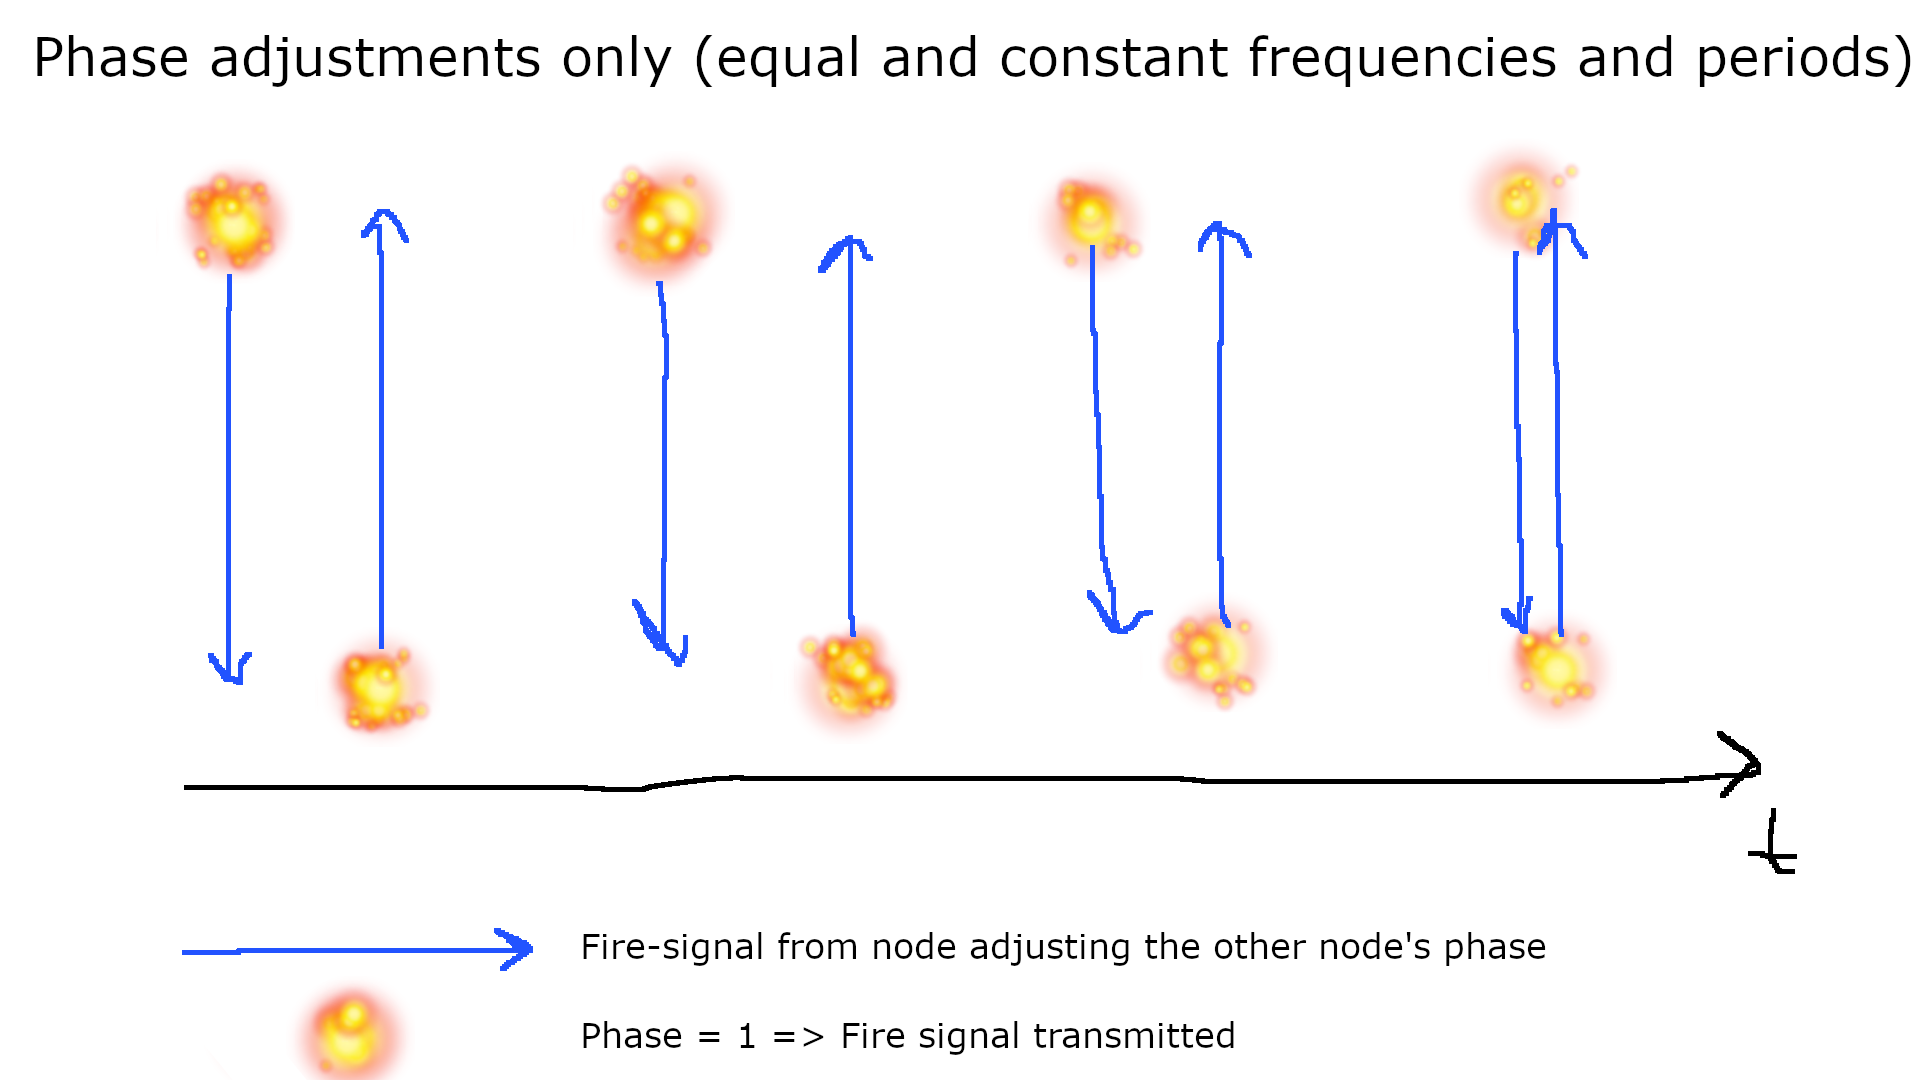
\includegraphics[width=0.90\textwidth]{Assets/Figures/phase_adjustments.png}
	\end{center}